\DiaryEntry{Group Theory}{2023-06-13}{Algebra}

The existing entries about group theory date back from 2016 and have various issues: (i) They are a bit too informal (as they are based on a introductory textbook), the topics repeat themselves and are spread across several entries (which themsevles are rather short in general). On a technical level, the entries were written in Pelican and have been converted to LaTex; some formatting issues arise from this conversion.

The idea is to rewrite and restructure the entries; I'm not sure whether that much is missing; the whole exercise is more about restructuring things.

I want to write new entries instead of rewriting the existing ones. The main reason is to preserve the history of the Journal.

\subsection{Introduction}

Groups are binary operations defined on a set. In addition, the set is closed under the binary operation. Let's start with some definitions.

\begin{definition}
A binary operation $\star$ on a set $G$ is a function $G \times G \rightarrow G$. For any $a, b \in G$ we write $a \star b$ when we combine them via this operation. 
\end{definition}


\begin{definition}
A group is an ordered pair $(G, \star)$ of a set $G$ and a binary operation $\star$. It satisfies the following axoims:

\begin{itemize}

\item The operation is associatvie; ie $(a \star b) \star c = a \star (b \star c)$ for all $a, b, c \in G$.
\item There exists an identity element $e \in G$ such that $a \star e = e \star a = a$ for all $a \in G$.
\item For each $a \in G$, there exists an inverse element $a^{-1}$ such that $a \star a^{-1} = e$.

\end{itemize}

The group is called abelian or commutative, if $a \star b = b \star a$ for all $a, b \in G$.

\end{definition}


Examples for groups are the numbers $\mZ$ with addition $+$ as binary operation. The addition is known / defined to be associative, the identity element is $0$, and the inverse for an element $a \in \mZ$ is given by $-a$. Another example are the rational numbers $\mQ$ with multiplication $\times$: The identity element is $1$ (as $1 \cdot a = a \cdot 1 = a$) and the inverse of $a$ is $\frac{1}{a}$.

A bit more tricky things happen when we consider addition modulo-$n$. Addition $\mod-n$ on a set of integers $G = \{0, 1, \cdots, n-1\}$ yields a group denoted as $\mZ / n \mZ$ with identitiy element $0$ and inverse element $n-a \equiv -a \mod n$. The multiplication table for $n = 5$ has the following structure.


\bee
\begin{array}{c|ccccc}
\star & 0 & 1 & 2 & 3 & 4 \\ \hline
0     & 0 & 1 & 2 & 3 & 4 \\
1     & 1 & 2 & 3 & 4 & 0 \\
2     & 2 & 3 & 4 & 0 & 1 \\
3     & 3 & 4 & 0 & 1 & 2 \\
4     & 4 & 0 & 1 & 2 & 3 \\
\end{array}
\eee

The first line repeats (in a shifted manner) in the lines below; this is a chracteristic of a \emph{cyclic group}; in addition, such a cyclic group can be created by repeatedly applying the group operation on the \emph{generator element}. The element $1$ is such a generator element and indeed we have

\bee
0 \star 1 = 1, 1 \star 1 = 2, 2 \star 1 = 3, 3 \star 1 = 4, 4 \star 1 = 0
\eee

As a last example, we again consider a set of integers $G = \{0, 1, \cdots, n-1\}$ but now with multiplication $\mod-n$ instead. The element $1$ acts as identitiy element $a \star 1 = 1 \star a = a$, but there is no inverse element for the element $0$: $a \star 0 = 0$ for all $a$. The way out of this is to remove the element $0$; ie we consider $G = \{1, 2, \cdots, n-1\}$ instead.

In the table below, the multiplication table of $G = \{1, 2, 3\}$ under multiplication $\mod-4$ is shown.

\bee
\begin{array}{c|ccc}
\star & 1 & 2 & 3 \\ \hline
1     & 1 & 2 & 3 \\
2     & 2 & 0 & 2 \\
3     & 3 & 2 & 1 \\
\end{array}
\eee

We can see that $0 \notin G$ appears in the second row and $2$ does not have an inverse - this is not a group! From the number theory entries and in particular theorem \ref{2020-11-25:th2}, we know that $a x \equiv 1 \mod n$ has a solution iff $\gcd(a,n) = 1$. So there are two ways to continue: (i) We remove all those elements $a$ from $G$ for which $\gcd(a,n) \neq 1$ or (ii) we consider only sets $G$ with prime cardinality (thereby trivially fulfilling the $\gcd(a,n) = 1$ condition).

Continuing way (i) in above example, we see that $2$ has $\gcd(2,4) = 2$ and we therefore must remove it from $G$. This results in the following multiplication table.

\bee
\begin{array}{c|cc}
\star & 1 & 3 \\ \hline
1     & 1 & 3 \\
3     & 3 & 1 \\
\end{array}
\eee

The alternative is to consider a set with a prime number of elements; "closest" is $n=5$ and for $G = \{1,2,3,4\}$ we have

\bee
\begin{array}{c|cccc}
\star & 1 & 2 & 3 & 4 \\ \hline
1     & 1 & 2 & 3 & 4 \\
2     & 2 & 4 & 1 & 3 \\
3     & 3 & 1 & 4 & 2 \\
4     & 4 & 3 & 2 & 1
\end{array}
\eee

No elements other than $G$ occur and every element has an inverse, so we have a group. We denote these groups as $(\mZ / n \mZ)^\times$.

A group possesses some further properties:

\begin{itemize}
  \item The identity element $e$ of a group is unique.
  \item For each $g \in G$, the inverse $g^{-1}$ is unique.
  \item $(g^{-1})^{-1} = a$, for all $g \in G$.
  \item $(a \star b)^{-1} = b^{-1} \star a^{-1}$.
  \item For any choice of $g_1, g_2, \ldots \in G$, the value of $g_1 \star g_2 \star \cdots$ is independent on the choice of bracketing.
\end{itemize}

The proofs follow from the group definition and is omitted.


\begin{definition}
  The \emph{order} of a group $G$, denoted $|G|$ is the number of its elements. The order of a group element $g$ is denoted by $|g|$ and is the smallest integer such that $g^n = e$.
\end{definition}

\subsection{Cyclic Groups}

In the examples above, we have seen that sometimes all group elements can be obtained by applying the group operation repeatedly on a specific element, the generator element $g$. That is $e, g, g \star g, g \star g \star g, \ldots$. For simpler notation, we write this as power expression; ie $g^0, g^1, g^2, \ldots$. Be careful as this denotes repeated application o the \emph{group operation} $\star$; in case the group operation is addition (modulo-$n$), $g^n$ is $n \cdot g$.

More formally,

\begin{definition}
    A group element $g \in G$ is a generator of the group $G$ if every element of $G$ can be expressed as power of $g$. A group $G$ is a cyclic group, if it can be generated by a single element, $G = \{g^n | n \in \mZ\}$. We also write $\langle g \rangle$ for the group.
\end{definition}

\paragraph{Generators of $\mZ / n \mZ$.} As example, we show that with $\mZ / n \mZ$ for $n=4$,

\begin{align*}
    &0 + 1 = 1, 1 + 1 = 2, 2 + 1 = 3, 3 + 1 = 0 \\
    &0 + 2 = 2, 2 + 2 = 0 \\
    &0 + 3 = 3, 3 + 3 = 2, 2 + 3 = 1, 1 + 3 = 0\\
\end{align*}

We can see that not every element is a generator; only $1$ and $3$ are. For a group element $g$ to be a generator, we must have $g^k = e$ for some integer $k$. Since we are using addition $\mod-n$, this is equivalent to $gk \equiv 1 \mod 1$ and from theorem \ref{2020-11-25:th2} we know that this happens only when $k$ is coprime to $n$.

\begin{theorem}
    A group element $g$ is a generator of $\mZ / n \mZ$, iff $g$ is coprime with $n$, or $\gcd(g, n) = 1$.
\end{theorem}

Proof: See above.

The number of integers coprime to $n$ is given by Euler's totient function $\phi(n)$; so there are $\phi(n)$ generators of $\mZ / n \mZ$.

\paragraph{Generators of $(\mZ / n \mZ)^\times$.} Let's start with the example from above, $(\mZ / 5 \mZ)^\times$ with elements $\{1, 2, 3, 4\}$ and loook at the powers of the elements.

\begin{align*}
    &1^2 = 1\\
    &2^2 = 4, 2^3 = 3, 2^4 = 1 \\
    &3^2 = 4, 3^3 = 2, 3^4 = 1 \\
    &4^2 = 1
\end{align*}

We see that the elements $2, 3$ are generators, the other two elements are not. As another example, consider $(\mZ / 8 \mZ)^\times$ with elements $\{1, 3, 5, 7\}$. The powers are

\begin{align*}
    &1^2 = 1 \\
    &3^2 = 1 \\
    &5^2 = 1 \\
    &7^2 = 1    
\end{align*}

This somewhat surprising result shows that this group does not have any generators.

\subsection{Dihedral Groups}

These groups, denoted by $D_n$, represent the rigid motions of a regular $n$-sided polygon. The groups have order $2n$. The groups are based on two operations, a rotation and a reflection, which also represent the generators of the group. A clockwise rotation operation $r$ is defined as follows:

\begin{figure}[H]
\centering
\includegraphics[scale=0.7]{images/groups_04_1.png}
\end{figure}

The reflection operation $s$ is defined as in the Figure below (depending on $n$ being even or odd, the reflection operation leaves one or two points unchanged).

\begin{figure}[H]
\centering
\includegraphics[scale=0.7]{images/groups_04_2.png}
\end{figure}

With these two generators, a Diheadral group $D_n$ is defined as all products of $r$ and $s$ which satisfy the following conditions:

\begin{align*}
r^n &= 1 \\
s^2 &= 1 \\
srs &= r^{-1}
\end{align*}

The first condition states, that after $n$ rotations all polygon points are back at their original position. The second  condition states that two reflections leave all polygon points unchanged. Finally, the third condition states, that the  sequence reflection-rotation-reflection is the same as rotation in the inverse direction.

So, more formally, we can define a Dihedral Group as follows.

\begin{definition}
    A Dihedral Group $D_n$ has two generators $r, s$ and the group has the following form.
    \bee
        D_n = \langle r, s | r^n = 1, s^2 = 1, srs = r^{-1} \rangle
    \eee
\end{definition}

This principle applies more generally: A group can be expressed as one more generators together with a set of \emph{relations}, which describe "simplifications" of certain elements. The general notation for such a description is as follows,

\bee
G = \langle g_1, g_2, \ldots | R_1, R_2, \ldots \rangle
\eee

where the $g_i$ are the generators and the $R_i$ are the relations. In the general case the group order is not obvious from the generators / relations as is the case if the Dihedral Group. \todo{include some stuff from Dummit, p. 26}

\subsection{Example $D_4$}

This group has $2n = 2 \dot 4 = 8$ elements. The identity element $e$, $3$ rotations $r, r^2, r^3$, one reflection $s$ and $3$ rotations preceded by a reflection $rs, r^2s, r^3s$. The choice of the last three elements is somewhat arbitrary (we could have used $sr, sr^2, sr^3$).

The elements are shown in the Figure below.

\begin{figure}[H]
\centering
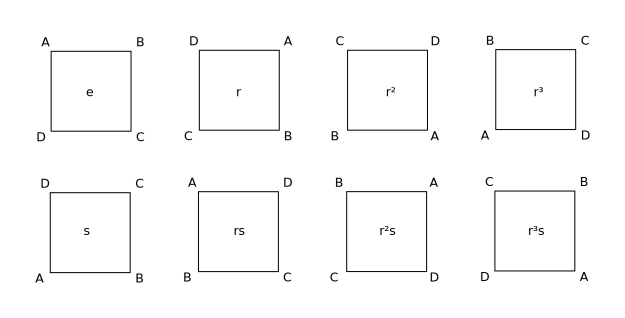
\includegraphics[scale=0.6]{images/groups_04_3.png}
\end{figure}

First note that the group is \textbf{not} abelian.

The multiplication table shall describe the relation between these $8$ elements; e.g. what is the result of $r^3s \star rs$. This can be simply written as $r^3srs$ but this expression is not in the form of one of the $8$ group elements. In order to achieve this, we need to simplify the resulting expressions so that they equal one of the elements.

The following multiplication table shows the results of multiplying elements without simplifying the result. All results in red need further simplification.

\[
\begin{array}{c|cccccccc}
\star   & 1    & r & r^2  & r^3 & s & rs & r^2s & r^3s \\
\hline
1 & 1 & r & r^2 & r^3 & s & rs & r^2s & r^3s \\
r & r & r^2 & r^3 & 1 & rs & r^2s & r^3s  & s \\
r^2 & r^2 & r^3 & 1 & r & r^2 s & r^3s & s & rs \\
r^3 & r^3 & 1 & r & r^2 & r^3s & s & rs & r^2s \\
s  &  s & \color{red}{sr} & \color{red}{sr^2} & \color{red}{sr^3} & e & \color{red}{srs}  & \color{red}{sr^2s} & \color{red}{sr^3s} \\
rs & rs & \color{red}{rsr} & \color{red}{rsr^2} & \color{red}{rsr^3} & r & \color{red}{rsrs}  & \color{red}{rsr^2s} & \color{red}{rsr^3s} \\
r^2s & r^2s & \color{red}{r^2sr} & \color{red}{r^2sr^2} & \color{red}{r^2sr^3} & r^2 & \color{red}{r^2srs}  & \color{red}{r^2sr^2s} & \color{red}{r^2sr^3s} \\
r^3s & r^3s & \color{red}{r^3sr} & \color{red}{r^3sr^2} & \color{red}{r^3sr^3} & r^3 & \color{red}{r^3srs} & \color{red}{r^3sr^2s} & \color{red}{r^3sr^3s}
\end{array}
\]

In order to simplify the red entries, we observe the following equalities:

\begin{itemize}
\item
  Start with $srs = r^{-1}$, left-multiply both sides with $s$ and obtain $s^2rs = s r^{-1}$ which becomes $rs = s r^{-1}$.   Righ-multiplying with $r$ finally yields $rsr = s$.
\item
  We have $sr = r^3 s$: Multiplying on the left with $r$, we obtain $rsr = r^4 s = r^3$. From the definitions above, we have $s = s$ which is true.
\item
  We have $sr^2 = r^2s$: Left-multiplying with $r$ yields $rsr^2 = r^3s$ which we can simplify to $sr = r^3s$ which was proven above.
\item
  We have $srs = r^{-1}$. Multiplying both sides with $r^4 = 1$, we obtain $srs = r^3$.
\end{itemize}

Finally, the table below shows the simplified multiplication table for the dihedral group $D_4$:

\[
\begin{array}{c|cccccccc}
\star   & 1    & r & r^2  & r^3 & s & rs & r^2s & r^3s \\
\hline
1 & 1 & r & r^2 & r^3 & s & rs & r^2s & r^3s \\
r & r & r^2 & r^3 & 1 & rs & r^2s & r^3s  & s \\
r^2 & r^2 & r^3 & 1 & r & r^2 s & r^3s & s & rs \\
r^3 & r^3 & 1 & r & r^2 & r^3s & s & rs & r^2s \\
s  &  s & r^3s & r^2s & rs & 1 & r^3  & r^2& r\\
rs & rs & s & r^3s& r^2s & r & 1  & r^3 & r^2\\
r^2s & r^2s & rs & s & r^3s & r^2 & r & 1 & r^3\\
r^3s & r^3s & r^2s & rs & s & r^3 & r^2 & r&  1
\end{array}
\]

The following Figure shows the corresponding Cayley diagram: Red lines correspond to multiplication with $r$ and blue lines correspond to multiplication with $s$. Since $s^2 = 1$ the orientation of the blue lines does \textbf{not} matter: Following a blue line in any direction \textbf{always} corresponds to multiplication by $s$ (This is contrary to multiplication with $r$ where the direction \textbf{is} important).

Note also that the Cayley diagram uses the convention that multiplication is interpreted from left to right; i.e. $A \star B$ corresponds to starting in point B, follow the line corresponding to multiplication with A. This can be seen in the right part: When we start at $r$ and follow the blue line to the inner circle, we land at the point $sr$ (which is equivalent to $r^3s$).

\begin{figure}[H]
\centering
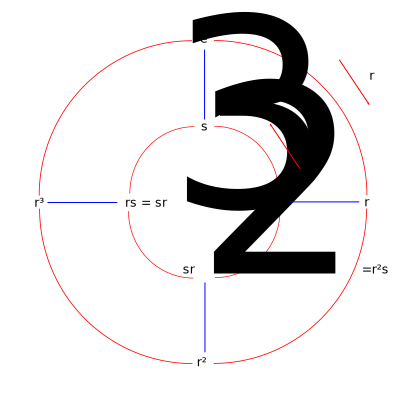
\includegraphics[scale=0.55]{images/groups_04_4.png}
\end{figure}

Using the more common convention that $AB$ corresponds to starting at $A$ and follow the line corresponding to  multiplication with $B$, we arrive at the Cayle diagram shown below. Again looking at the right part of the Figure, when we start at $r$ and follow the blue line to the inner circle, we land at the point $rs$.

\begin{figure}[H]
\centering
\includegraphics[scale=0.55]{images/groups_04_5.png}
\end{figure}

\subsection{Permutations / Symmetric Groups}

The permutations of a set form a group: Let $A$ be a set and $S_A$ be the set of all bijections from $A$ onto itself. Then $S_A$ is a group under function decomposition $\star$. This is a binary operation, because if$\sigma$ and $\tau$ are both bijections from $A$ onto $A$, so is their combined action $\sigma \star \tau$. Function composition is associative in general, therefore als in this case. The identity element $e$ is the "identity" permutation $e \star a = a$ for all $a \in A$ and for every permutation $\sigma$ there is an inverse function $\sigma^{-1}$ which reverses $\sigma$, so we have $\sigma \star \sigma^{-1} = e$. This group is called the symmetric group on the set $A$. It is important to recognize that the elements of $S_A$ are permutations of $A$ and \emph{not} the elements $A$ themselves.

We will mostly consider the case that $A = \{1, 2, \ldots, n\}$ in this case the symmetric group is denoted by $S_n$. It has order $n!$ as there are $n!$ different permutations of $n$ elements.

The simplest (and most verbose) way of describing permutations is by writing down what the permutation does with each element; eg. in form of a table (linking input with output values). This can look as follows.

\[
\sigma =
\begin{pmatrix}
1 & 2 & 3 & 4 & 5 \\
1 & 2 & 3 & 5 & 4
\end{pmatrix}
,\quad \tau = 
\begin{pmatrix}
1 & 2 & 3 & 4 & 5 \\
2 & 3 & 1 & 4 & 5
\end{pmatrix}
, \quad \mu = 
\begin{pmatrix}
1 & 2 & 3 & 4 & 5 \\
2 & 3 & 1 & 5 & 4
\end{pmatrix}
\]

Permutation $\tau$ does not change elements $1, 2, 3$, but exchanges $4$ and $5$. Permutation $\tau$ (cyclically) moves $1, 2, 3$, leaving $4, 5$ unchanged. Finally, permutation $\mu$ (cyclically) moves $1, 2, 3$, and exchanges $4$ and $5$.

\paragraph{Cycle Notation.} From above examples we can see that permutations either do not affect elements or exchange / move them around. Repeated application of the same permutation creates \emph{cycles} and it turns out that we can characterize a permutation by its cycles. We use a special notation for writing down cycles: Elements belonging to a cycle are written in brackets and the cycles (if there are several) are written next to each other. For example, a permuation $(1,3,5)(2,4)$ has two cycles, one with $3$ elements and on with $2$ elements.

Cycles with one element are not written down; the shortest cycle is one of length $2$ and called a \emph{transposition}. The length of a cycle is the number of integers that appear in it. A cycle of length $t$ will be called $t$-cycle.

Note that the order of the elements in the cycle is important; i.e. cycles $(1,2,4,3)$ and $(1,2,3,4)$ denote different cycles. However, we can "rotate" elements in the cycle expression; so do $(1,2,3), (2,3,1), (3,1,2)$ all represent the same permutation.

To move from a table like above to cycle notation, we make use of the \emph{cycle decomposition algorithm}. It starts with the smallest element not yet appeared in a cycle and "follows" the element along a cycle. This creates the first cycle. Then the algorithm picks the next unused integer and repeats the following, creating the next cycle. When all integers are used up, the algorithm terminates.

In the permutation $\sigma$ in the example above, $\sigma(1) = 1, \sigma(2) = 2, \sigma(3) = 3$ which corresponds to three  $1$-cycles which we do not write down. Continuing with $4$, we have $\sigma(4) = 5$, so we start a cycle with $(4, 5$. Since $\sigma(5) = 4$, we are back at the starting point and close the cycle to obtain $(4,5)$. Since we have used up all integers, we are done, and the permutation can be expressed as $(4,5)$.

In the permutation $\tau$, we start with $1$ and $\tau(1) = 2$. We therefore start a cycle $(1,2$. Continuing, we have $\sigma(2) = 3$, and $\sigma(3) = 1$, so we have a cycle $(1,2,3)$. Since $\tau(4) = 4$, and $\tau(5) = 5$, we have no further cycle and $\tau$ can be expressed as $(1,2,3)$.

Finally, $\mu$ has one cycle $(1,2,3)$ (like $\tau$ above). However, we have $\mu(4) = 5$ and $\mu(5) = 4$, so we have another cycle and the permutation can be expressed as  $(1,2,3)(4,5)$.

\paragraph{Permutation Composition.} The group operation (permutation composition) becomes rather simple with the cycle presentation as is shown in the following. 

For example if we have $\sigma=(1,3,5,2)$ and $\tau = (2,5,6)$, then the composition $\sigma \tau$ can be obtained by considering the effect of $\sigma \tau$ on every integer: We have

\begin{align*}
  &\sigma (\tau (1)) = \sigma(1) = 3 \\
  &\sigma (\tau (2)) = \sigma(5) = 2 \\
  &\sigma (\tau (3)) = \sigma(3) = 5 \\
  &\sigma (\tau (4)) = \sigma(4) = 4 \\
  &\sigma (\tau (5)) = \sigma(6) = 6 \\
  &\sigma (\tau (6)) = \sigma(2) = 1
\end{align*}

Converting this into cycle notation, we obtain for the product $\sigma \star \tau = (1,3,5,2) \star (2,5,6) = (1,3,5,6)$. Note, that the composite permutation does not change the elements $2$ and $4$; the element $2$ is not affected by neither $\sigma$ nor $\tau$, whereas the element $4$ is affected by both $\sigma$ and $\tau$.

If we exchange order of permutations, we obtain $\tau \star \sigma = (2,5,6) \star (1,3,5,2) = (1,3,6,2)$ from which we see that composition is \emph{not} commutative.

We can check on this in Gap, however, we must be careful as Gap uses left-to-right application. So we have

\begin{verbatim}
    gap> (2,5,6)*(1,3,5,2);
    (1,3,5,6)
    gap> (1,3,5,2)*(2,5,6);
  (1,3,6,2)
\end{verbatim}

\paragraph{Cycle Identities.} There are some rules / simplifications which can be helpful. A \emph{transposition} is a cylce of length 2, $(a,b)$ which we can  also interpret as an element exchange. The inverse of a transposition is the transposition itself; i.e.

\bee
(a,b)^{-1} = (a,b)
\eee

The inverse of longer cycles has also a simple form, namely

\bee
(a_1,a_2, \ldots, a_N)^{-1} = (a_1, a_N, a_{N-1}, \ldots a_{2})
\eee

Two cycles are \emph{disjoint} if they contain different elements. If $\sigma$ and $\tau$ are disjoint cycles, then $\sigma \tau = \tau \sigma$. Multiplication of two disjoint cycles becomes

\bee
(a_1, a_2, \ldots, a_N) \star (b_1, b_2, \ldots, b_M) = (a_1, a_2, \ldots, a_N) (b_1, b_2, \ldots, b_M)
\eee


\begin{theorem}
Every permutation can be epxressed as product of disjoint cycles. This representation is unique up to the rearrangement of the cycles.
\end{theorem}

Proof is omitted.

In a similar spirit, we can express longer cycles as product of transpositions, eg

\bee
(1,2,3) = (1,3)(1,2)
\eee

This raises the question whether all permutations can be expressed as product of transpositions. This is indeed the case. We first observe that we can split any $m$-cycle into a product of transpositions as follows,

\bee
(a_1, a_2, \ldots a_N) = (a_1, a_m)(a_1, a_{m-1}) \cdots (a_1, a_2)
\eee

Now any permutation can be written as product of disjoint cycles and therefore, we can write every permutation as product of transpositions, or equivalently,

\bee
S_n = \langle T \rangle, \quad T = \{(i,j) | 1 \leq i < j \leq n\}
\eee

As an example, we have

\bee
(1,2,7)(4,5)(6,8,10,9) = (1,7)(1,2)(4,5)(6,9)(6,10)(6,8)
\eee

Note, however, that the representation is not unique \todo{show example}

However, we can define the \emph{parity of a permutation} which is the same for any representation of the permutation.

Define a polynomial $\Delta$ in the variables $x_1, \ldots, x_n$ as follows,

\bee
\Delta = \prod_{1 \leq i < j \leq n} (x_i - x_j)
\eee

For example, for $n=4$ we obtain the polynomial $\Delta = (x_1 - x_2)(x_1 - x_3)(x_1 - x_4)(x_2 - x_3)(x_2 - x_4)(x_3 - x_4)$. Now we let a permutation $\sigma$ operate on the polynomial $\Delta$ by permutating its indices:

\bee
\sigma(\Delta) = \prod_{1 \leq i < j \leq n} (x_{\sigma(i)} - x_{\sigma(j)})
\eee

If we choose $\sigma = (1,2,3,4)$ and apply this to the polynomal defined above, we obtain

\bee
\sigma(\Delta) = (x_2 - x_3)(x_2 - x_4)(x_2 - x_1)(x_3 - x_4)(x_3 - x_1)(x_4 - x_1)
\eee

We see that $\sigma(\Delta)$ has the same terms as $\Delta$, however, sometimes the order of variables is reversed (in our example, this is eg $(x_1 - x_2)$). We can revert the original order by inserting a factor $(-1)$ (in the example, $(-1)(x_2 - x_1)$) and we therefore have

\bee
\sigma(\Delta) = \pm \Delta
\eee

We define the \emph{parity or sign} $\epsilon$ of the permuation $\sigma$ as

\bee
\epsilon(\sigma) = \begin{cases} &+1, \text{ if } \sigma(\Delta) = \Delta \\
-1, \text{ if } \sigma(\Delta) = -\Delta \end{cases}
\eee

In our running example, the order of variables is reversed three times and therefore

\bee
\sigma(Delta) = (-1) \Delta
\eee

and therefore the parity of $\sigma = (1,2,3,4)$ is $\epsilon((1,2,3,4)) = -1$.

\begin{definition}
The quantity $\epsilon(\sigma)$ is called the parity or sign of a permutation. A permutation is called even, if $\epsilon(\sigma) = 1$, otherwise it is odd.
\end{definition}

We can obtain the sign in Gap as follows.

\begin{verbatim}
  gap> s:=(1,2,3,4);
  (1,2,3,4)
  gap> SignPerm(s);
  -1
\end{verbatim}

which matches the calculation we did above. \qed

The set of even permuations is a group under permutation composition and is called the \emph{alternating} group $A_n$.

Futhermore, we have the following theorem.

\begin{theorem}
The alternating group $A_n$ is a non-abelian group for $n \geq 5$.
\end{theorem}

Proof is omitted.


\subsection{Group Actions}

A permutation is an element of the symmetric group and acts on elements from a set. It is important to distinguish between the permutation itself (eg $(1,2,3)$) and the element it actos upon (eg $2$): $(1,2,3) 2 = 3$.

\begin{definition}
A \emph{group action} of a group $G$ on a set $A$ is a map from $G \times A$ to $A$, written as $g \cdot a$ (with $g \in G, a \in A$) satisfying the following properties:
\begin{itemize}
\item $g_1 \cdot (g_2 \cdot a) = (g_1 g_2) a$ for all $g_1, g_2 \in G$ and $a \in A$ and
\item $1 \cdot a = a$ for all $a \in A$.
\end{itemize}
\end{definition}

If we fix $g$, then we get a map $\sigma_g: A \rightarrow A$ with $\sigma_g(a) = g \cdot a$ and we can show that this map $\sigma_g$ is a permutation of $A$ (proof omitted).

Intuitively, a group action of $G$ on a set $A$ just means that every element $g \in G$ acts as a permutation on $A$ in a manner consistent with the group operations in $G$.

%%% Local Variables:
%%% mode: latex
%%% TeX-master: "journal"
%%% End:
